% !TeX spellcheck = en_GB

\section{\Pi{}}
In Chinese, \Pi{} \begin{CJK*}{UTF8}{bsmi}劈\end{CJK*} means \textit{to split}, \textit{to cut} but also \textit{to hit}, \textit{to go straight to}. In essence, \Pi{} is a splitting cut that goes straight through the target.

As a basic technique, \Pi{} is simply described as a downward vertical splitting cut. It is often associated with an outside or inside whirl of the sword, which I will not describe here in detail as it is actually not part of the \Pi{} technique and will be more appropriately explained elsewhere.

Although the formal \Pi{} technique is a downward cut,  I personally think that the \Pi{} splitting energy can be oriented in any direction. Thus, even horizontal or upward cuts which characteristically split the target open without any slicing movement may somehow be considered akin to this energy.

The formal emblematic \Pi{} technique is prepared by raising the sword handle up to ear level while sinking into the leg opposite to the armed hand. The grip should be relaxed yet firmly secured between the middle fingers and the thumb. The other fingers maintain a relaxed contact with the handle allowing some flexibility in the grip while at the same time keeping control of the blade. 
In a less formal, less static context, this preparation would be combined with footwork while parrying or evading an attack, seamlessly transforming the defensive action into the riposte.

During the first phase of the cut, the hand is thrown downwards along a diagonal, drawing the sword forwards and downwards in the direction of the pommel to accelerate the blade. The slanted force the hand exerts on the handle, combined with the action of the last two fingers tightening their grip, makes the sword to gradually rotate around its centre of gravity (fig. \ref{fig:pi_cut} a).

This movement draws its energy from the expansion of the body, which may be seconded by a forward step for increased reach and cutting power. 

Then, once the hand has been overtaken by the sword's centre of gravity (fig. \ref{fig:pi_cut} b), it stops exerting an action and simply follows the handle, while keeping a relaxed yet firm control of the sword's trajectory. Thus, the blade is moving freely when it reaches the target with an unperturbed trajectory, and all the kinetic energy accumulated during the acceleration phase is fully transferred into the cut (fig. \ref{fig:pi_cut} c).

\begin{figure}[ht]
\centering
	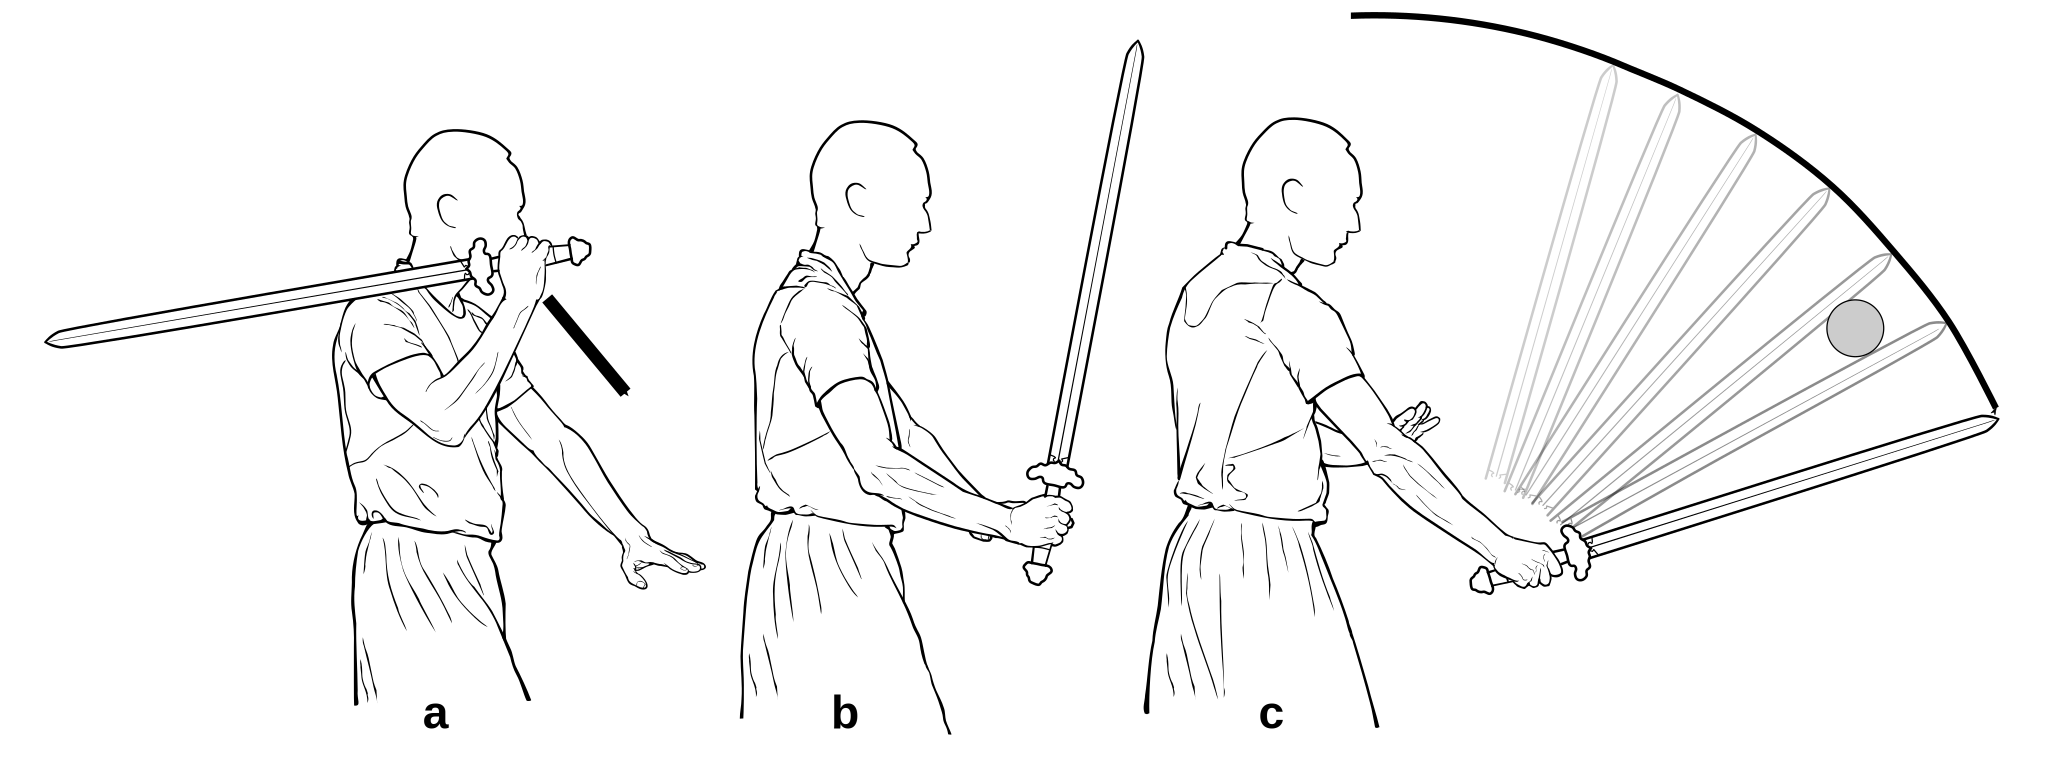
\includegraphics[width=1.00\textwidth]{../../Images/JibenJianfa/Pi/Pi_juxtaposed.pdf}
	\caption[\Pi{} cut]{\Pi{} cut: (a) Starting from a high position of the sword, the right hand draws the sword handle downwards to accelerate the blade; (b) shows the end of the acceleration phase, from now on, the hand will not exert any more action on the handle; (c) the hand follows the handle with only a firm control of the sword's trajectory so that the blade is allowed to move freely though the target represented here by a grey circle. Note that the trajectory of the blade tip is not circular but an elongated arc.}
	\label{fig:pi_cut}
\end{figure}

It is absolutely crucial that the flat is perfectly aligned with the blade trajectory to make sure that the weight of the blade lies behind the edge to push it through the target. If the blade hits the target at an angle, no matter how small, it tends to rotate on its axis and may bounce back dangerously instead of nicely cutting through the target. On the other hand, when the alignment is correct and the grip is relaxed, the blade will flash through the target without any appreciable feedback. 

After the cut, the handle naturally presses against the heel of the hand and all the fingers tighten their grip to bring the sword to a halt at waist level in a protective position without any tension nor bounce. Thanks to a proper body alignment, the sword's energy is thus returned to the body, helping to recentre oneself and make ready for the next technique.

\fiche{ 
training tips and drills
figures: the whole technique,  blade alignment with trajectory

combination of the  sword rotation and the forward movement of the hand.
unwinding movement with extension to the front like angling but with a downward direction as well.
splitting,  short,  often done at the beginning of other cuts such as Hua generally performed in a downward direction, but may be oriented towards any direction 
}

